\documentclass[lettersize,journal]{IEEEtran}
\usepackage{amsmath,amsfonts}
\usepackage{algorithmic}
\usepackage{algorithm}
\usepackage{array}
\usepackage[caption=false,font=normalsize,labelfont=sf,textfont=sf]{subfig}
\usepackage{textcomp}
\usepackage{stfloats}
\usepackage{url}
\usepackage{verbatim}
\usepackage{graphicx}
\usepackage[dvipdfmx]{graphicx}
\usepackage[dvipdfmx]{color}
\usepackage{cite}
\hyphenation{op-tical net-works semi-conduc-tor IEEE-Xplore}

\begin{document}

\title{OUXT Polaris: Autonomous Navigation System for the 2022 Maritime RobotX Challenge}
\author{
    Kenta Okamoto,Kyoto Institute of Tech., m2623106@edu.kit.ac.jp \\ \and
    Akihisa Nagata, Kansai Univ. , k065604@kansai-u.ac.jp \\ \and
    Masato Kobayashi, Kobe Univ. , 171w951w@gsuite.kobe-u.ac.jp \\ \and
    Shunya Tanaka, , syun111@gmail.com \\ \and
    Masaya Kataoka, TEIR IV inc . , ms.kataoka@gmail.com,
}

% The paper headers
\markboth{IEEE TRANSACTIONS ON XXXXX,~Vol.~xx, No.~x, XXX~2022}%
{Shell \MakeLowercase{\textit{et al.}}: A Sample Article Using IEEEtran.cls for IEEE Journals}

% \IEEEpubid{0000-0000/00\$00.00~\copyright~2021 IEEE}
% Remember, if you use this you must call \IEEEpubidadjcol in the second
% column for its text to clear the IEEEpubid mark.

\maketitle

\begin{abstract}
OUXT-Polaris has been developing an autonomous navigation system by participating in the 
Maritime RobotX Challenge 2014, 2016, and 2018. 
In this paper, we describe the improvement of the previous vessel system. 
We also indicate the advantage of the improved design.
Moreover, we describe the developing method for Covid-19 and the 
feature components for the next RobotX Challenge.
\end{abstract}

\begin{IEEEkeywords}
Maritime systems, Robotics, Unmanned surface vehicle
\end{IEEEkeywords}

\section{Introduction}
First of all, we are motivated to develop a big field robot in a large area such as the ocean.
In recent years, the aging and shrinking population, as well as a shortage of workers,
has led to an increase in demand for the automation of cars, robots, and other equipment.
Among these, automated driving is being developed with particular emphasis.
Moving the autonomous vehicle or robot outside has a very severe problem.
They need to hedge unknown obstacles and go to the target position.
The environment such as weather, temperature, or underwater around robots causes sensor and hardware problems.
There are each challenging problems and They are also interesting for us.  
In this competition, we have a chance to develop a system to get over the wild environment 
for the robots on the ocean. Therefore, we are participating in the Maritime RobotX Challenge.


\section{MINI-V in the COVID-19}
MINI-V(minitua vessel) was created in order to test the software easily in the Covid-19. Over the past several years, 
we couldn't conduct the experiment on the ocean or lake because of the COVID-19.
We were prohibited to meet and create the parts of WAM-V.
 In addition, the law about vessels is very strict.
So, we can't float the boat easily. The WAM-V is so big and it is hard work and costs too much to carry WAM-V to the lake. 
Then, we need a sustainable system to develop the automotive vessel.
As mentioned above, the simulator is used for developing navigation systems, and it doesn't need to use WAM-V.
The perception array was created to get the sensor data for software tests. They made it easier for us to develop software without ships.
 However, the software and hardware integration is the most important to conduct tasks. Then, MINI-V was created 
to make it easier to do the test and the integration.

The concepts of MINI-V are follows:
\begin{enumerate}
  \item easy assembly, transport, and experiment,
  \item open source software and hardware,
  \item high compatibility between WAM-V and MINI-V.
\end{enumerate}
MINI-V is created to be easy to carry, and we can carry them by suitcase like Fig. (b). 
It is also assembled simply. We develop this vessel on open source. So, other people can play or test their software with MINI-V. Finally,
we expect the high compatibility between WAM-V and MINI-V, and it will make it easy to migrate developed software on MINI-V toWAM-V. However, 
MINI-V have not had complete compatibility yet.
We have future tasks to create a little bigger vessel to have compatible hardware and software such as batteries and sensors, and so on.

% \begin{figure}[ht]
%   \begin{minipage}[b]{\linewidth}
%       \centering
%       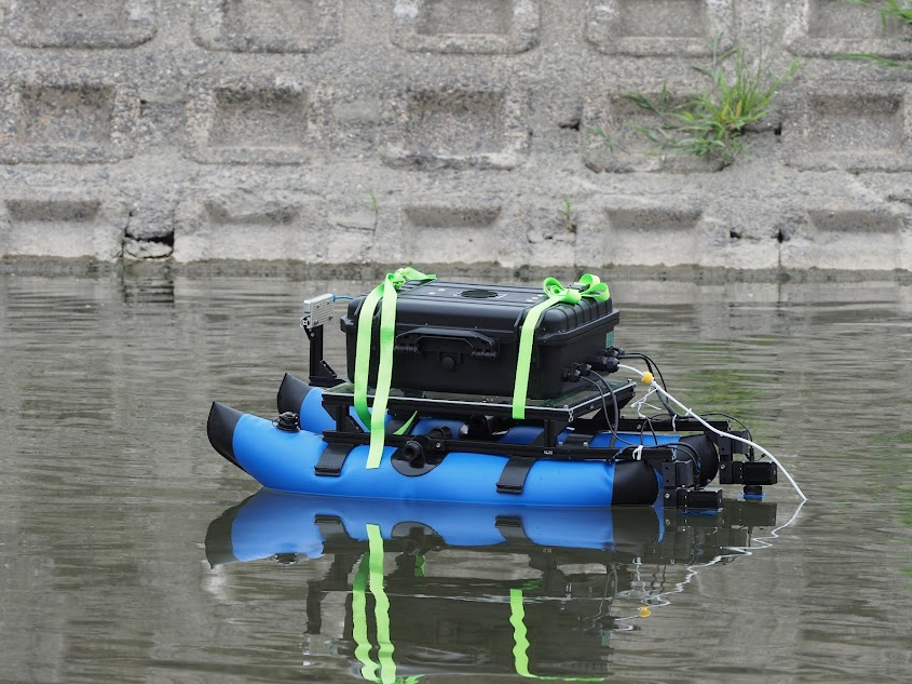
\includegraphics{figure/mini_v_overview.png}
%       \subcaption{the experiment on the river}
%       \label{fig:mini-v1}
%   \end{minipage}
%   \begin{minipage}[b]{\linewidth}
%       \centering
%       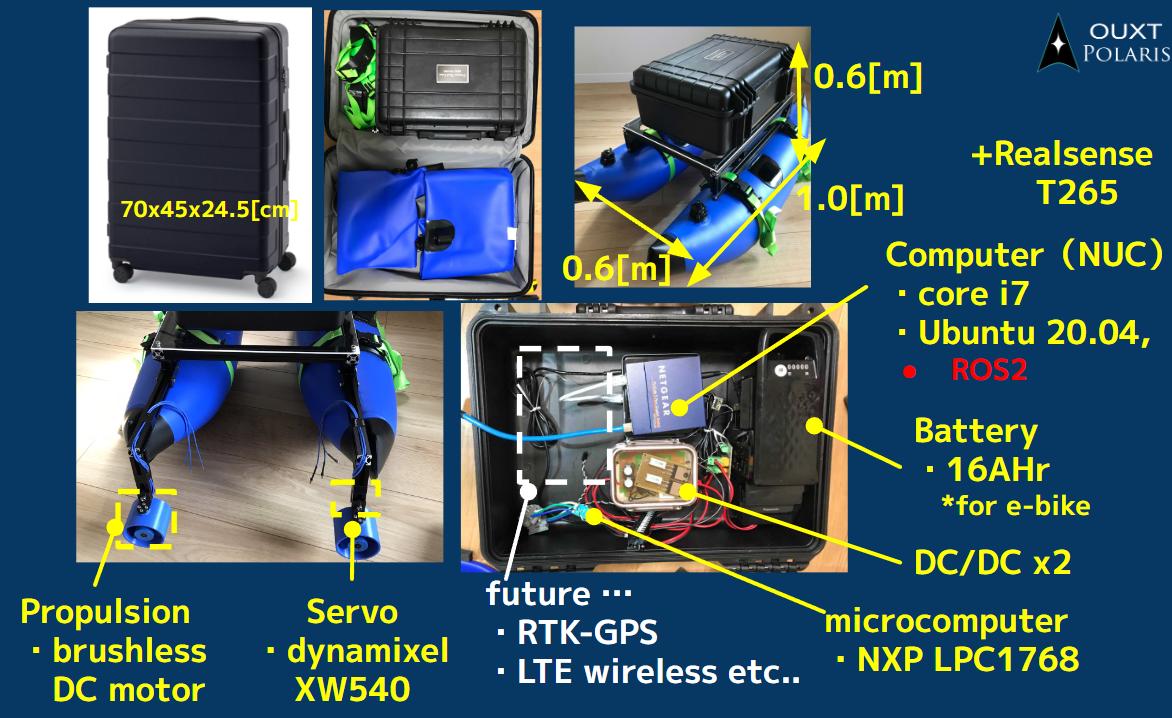
\includegraphics{figure/mini_v_component.png}
%       \subcaption{the components of MINI-V}
%       \label{fig:mini-v2}
%   \end{minipage}
%   \caption{the overview of MINI-V}
% \end{figure}

\section{Conclusion}
XXXXXX
% \section*{Acknowledgments}
\begin{thebibliography}{1}
\bibliographystyle{IEEEtran}

  \bibitem{YOLOX}
  Ge, Zheng, et al. "Yolox: Exceeding yolo series in 2021." arXiv preprint arXiv:2107.08430 (2021).

  \bibitem{RobotX2018_video}
  \url{https://www.youtube.com/watch?v=MqDBxzS4uy4}

\end{thebibliography}

\vfill

\end{document}